% Course-project draft. Compile with pdflatex + bibtex (Overleaf default).
\documentclass[11pt,a4paper]{article}
\usepackage[margin=2.3cm]{geometry}
\usepackage[T1]{fontenc}
\usepackage{lmodern,microtype}
\usepackage{amsmath,amssymb,physics}
\usepackage{graphicx,booktabs,xcolor,tabularx}
\usepackage{caption}
\usepackage[section]{placeins}

\usepackage[numbers,sort&compress]{natbib}
\usepackage[colorlinks,linkcolor=blue,citecolor=blue,urlcolor=blue]{hyperref}
\hypersetup{pdftitle={Quantum-Circuit-Based Solution of Ordinary and Partial Differential Equations (draft)},pdfauthor={Mushrafi Munim Sushmit}}
\captionsetup{font=small,labelfont=bf}
\setlength{\emergencystretch}{2em}
\setcounter{topnumber}{3}
\renewcommand{\topfraction}{0.9}
\renewcommand{\textfraction}{0.08}
\renewcommand{\floatpagefraction}{0.7}
\title{Quantum-Circuit-Based Solution of\\ Ordinary and Partial Differential Equations}
\author{Mushrafi Munim Sushmit\\[2pt]
\small Department of Physics and Astronomy, University of Tennessee, Knoxville\\[4pt]
\small Course project, Physics 610: Quantum Optics and Quantum Information Science, Fall 2026\\
\small Instructors: Haocun Yu and George Siopsis}
%\date{Draft, October 26, 2026}
\begin{document}
\maketitle
\section{Project overview}\label{sec:overview}
This project studies how parameterized quantum circuits can be used as trainable
function approximators for solving ordinary and partial differential equations
within a physics-informed framework~\cite{raissi2019,cerezo2021vqa,cerezo2022qml}.
As in classical physics-informed neural networks, the governing differential
equation and its initial or boundary conditions are incorporated into a loss
function. The unknown solution is represented by the expectation value of a
parameterized quantum circuit, and derivatives of the circuit output are
evaluated with differentiable quantum-circuit techniques~\cite{kyriienko2021}.
Recent work has developed this idea with trainable embeddings~\cite{teqpinn2025},
formulations for multivariable partial differential equations~\cite{panichi2026},
and Lagrange-polynomial encodings~\cite{hunout2025}. The learned solutions are
compared with known analytical or reference solutions.

\section{Method}\label{sec:theory}
\subsection{A circuit as a trial solution}
Following Kyriienko \emph{et al.}~\cite{kyriienko2021}, the trial solution is a
circuit expectation value. An encoding block $S(t)$ loads the input and a
trainable block $W(\boldsymbol\theta)$ follows:
\begin{equation}
 \ket{\psi(t;\boldsymbol\theta)}=W(\boldsymbol\theta)S(t)\ket0^{\otimes n},
 \qquad f(t;\boldsymbol\theta)=\ev{Z_0}{\psi(t;\boldsymbol\theta)}.
\end{equation}
Since $f\in[-1,1]$, it is mapped onto a readout scaling $[\ell,h]$ chosen around the
expected solution range:
\begin{equation}
 u_\theta(t)=\ell+a\,[1+f(t;\boldsymbol\theta)],\qquad a=\frac{h-\ell}{2}.
 \label{eq:model}
\end{equation}

A differential equation on a domain $\mathcal D$ with conditions on a set
$\Gamma$ can in general be written as
\begin{equation}
 \mathcal N[u](x)=0,\quad x\in\mathcal D,\qquad\qquad
 \mathcal B[u](x)=g(x),\quad x\in\Gamma,
 \label{eq:ode}
\end{equation}
e.g.\ for Rabi oscillations $\mathcal N[u]=u''+\Omega^2u-\Omega^2/2$ on
$[0,2\pi]$ with $\mathcal B[u]=(u(0),u'(0))$ and $g=(0,0)$. Since the residual
\begin{equation}
 \mathcal R_\theta(x)=\mathcal N[u_\theta](x)
 \label{eq:residual}
\end{equation}
vanishes when $u_\theta$ solves the equation. If we optimize the circuit parameters over $M$
collocation points and $B$ condition points~\cite{raissi2019,kyriienko2021},
\begin{equation}
 \mathcal L(\boldsymbol\theta)=
 \underbrace{\frac1M\sum_{m=1}^{M}\mathcal R_\theta(x_m)^2}_{\text{residual loss}}
 +\underbrace{\frac1B\sum_{b=1}^{B}\bigl\|\mathcal B[u_\theta](x_b)-g(x_b)\bigr\|^2}_{\text{condition loss}}.
 \label{eq:loss}
\end{equation}
We can train the quantum circuit to represent the solution of the differential equation. No solution data is needed for the loss but can also be included if available. In this work, we will not use any solution data. (Fig.~\ref{fig:workflow}).
\begin{figure}[htbp]
\centering
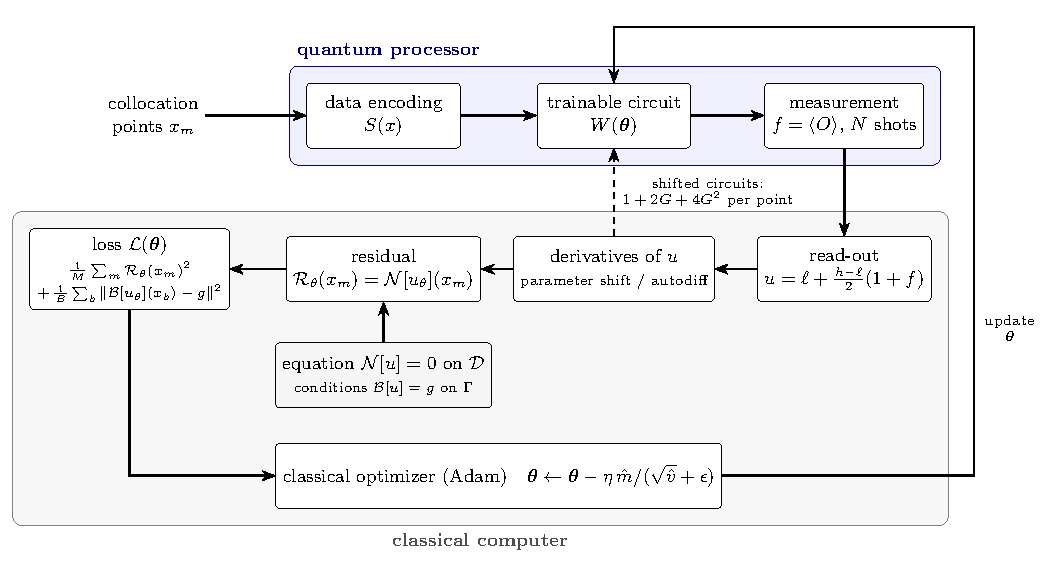
\includegraphics[width=\linewidth]{diagrams/qpinn_workflow.pdf}
\caption{Training loop: the circuit gives $u_\theta$ and its derivatives, the equation and conditions define the loss, and a classical optimizer updates $\boldsymbol\theta$.}
\label{fig:workflow}
\end{figure}

\subsection{Derivatives on hardware}
To generate the differential equation, we will need to find the derivative to construct the differential equation from the expectation value of the quantum circuit. In this simulations, we use automatic differentiation scheme. On hardware, derivatives follow from the parameter-shift rule~\cite{mitarai2018,schuld2019},
\begin{equation}
 \partial_\phi f=\frac12\left[f(\phi+\pi/2)-f(\phi-\pi/2)\right].
 \label{eq:ps}
\end{equation}
With encoding angles
\begin{equation}
 \phi_g=c_g\,t,
\end{equation}
the chain rule gives
\begin{align}
 f'&=\sum_g c_g\,\partial_{\phi_g}f,\label{eq:ps1}\\
 f''&=\sum_{g,h}c_gc_h\,\partial_{\phi_g}\partial_{\phi_h}f,\label{eq:ps2}
\end{align}
so $G$ encoding gates cost
\begin{equation}
 N_{\rm eval}=1+2G+4G^2
\end{equation}
circuit evaluations per point for $(f,f',f'')$.

\subsection{Four trial-function architectures}

Since random parameterized quantum circuits often suffer from severe trainability issues such as barren plateaus, we utilize structured circuit families documented in the literature.

Here, We compare four circuit families (Fig.~\ref{fig:circuits}), each a
variational quantum circuit in the sense of Ref.~\cite{cerezo2021vqa}. The first
two encode the input once and differ only in their trainable gates; the other
two upload the input again in every layer. Every model measures the first qubit
and is mapped to the solution by Eq.~\eqref{eq:model}.

\paragraph{M{\o}lmer--S{\o}rensen (MS) ansatz.}
The input is encoded once on every qubit, followed by repeated layers of
general single-qubit rotations and nearest-neighbour two-qubit $XX$ gates. The
$XX$ gate is the M{\o}lmer--S{\o}rensen interaction, generated by a
spin-dependent force on the shared motion of trapped ions~\cite{molmer1999,sorensen1999},
so every gate is native to trapped-ion hardware~\cite{bruzewicz2019}. The layout
is our trapped-ion adaptation of a layered variational circuit.

\paragraph{Hardware-efficient ansatz (HEA).}
The same single encoding is followed by a fixed body of Hadamard and rotation
layers separated by chains of CNOT gates, following the strategy of combining
simple rotations with readily available entanglers~\cite{kandala2017draft}.
Since MS and HEA share the encoding, comparing them asks how much the trainable
structure matters on its own.

\paragraph{Data re-uploading.}
Following P\'erez-Salinas \emph{et al.}~\cite{perezsalinas2020}, the input
re-enters before every layer, with a coefficient that grows with depth. Each
layer applies single-qubit rotations and CNOT chains, and the first qubit is
measured directly after the last layer.

\paragraph{Trotterized Ising ansatz.}
The input is re-uploaded as in data re-uploading, but each trainable block is a
Trotter--Suzuki product-formula approximation~\cite{suzuki1991} to evolution
under an Ising-type Hamiltonian with trainable $ZZ$ and $XX$ couplings and local
fields, using two Trotter steps. Every factor is a native two-qubit or
single-qubit gate, the sequence of digital quantum simulation~\cite{lloyd1996}
as run on trapped ions~\cite{lanyon2011}. Here the product formula defines the
variational family; it does not approximate a prescribed target evolution.

\begin{figure}[p]
\centering
\begin{tabular}{@{}p{\linewidth}@{}}
\textbf{(a)} MS ansatz (trapped-ion native)\\
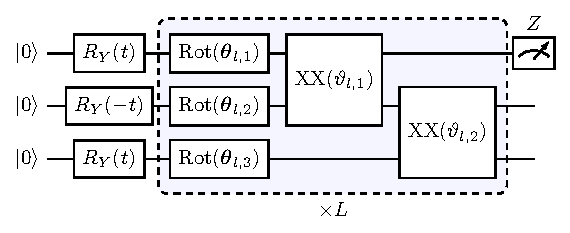
\includegraphics[width=0.55\linewidth]{diagrams/ms.pdf}\\[6pt]
\textbf{(b)} Hardware-efficient ansatz (HEA)\\
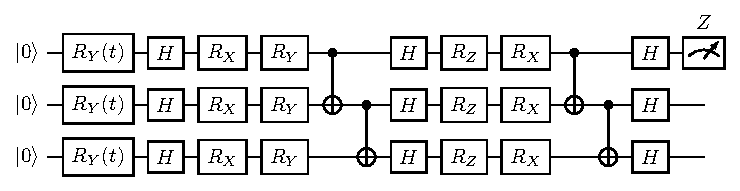
\includegraphics[width=0.85\linewidth]{diagrams/hea.pdf}\\[6pt]
\textbf{(c)} Data re-uploading\\
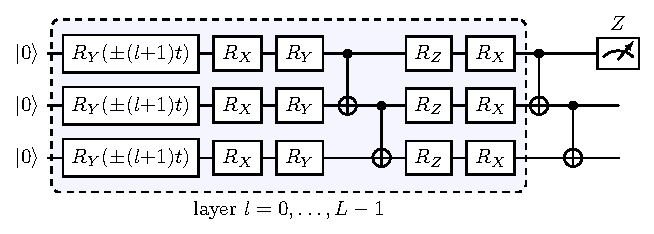
\includegraphics[width=0.85\linewidth]{diagrams/reupload.pdf}\\[6pt]
\textbf{(d)} Trotterized Ising-Hamiltonian ansatz, and one Trotter step ($\delta=\tau/s$)\\
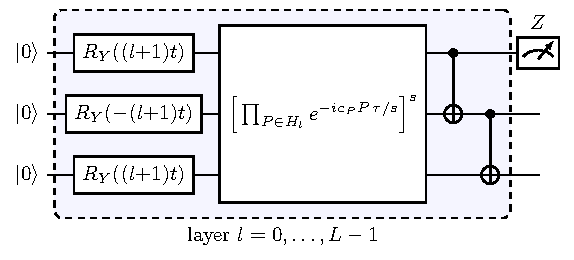
\includegraphics[width=0.42\linewidth]{diagrams/trotter.pdf}\hfill
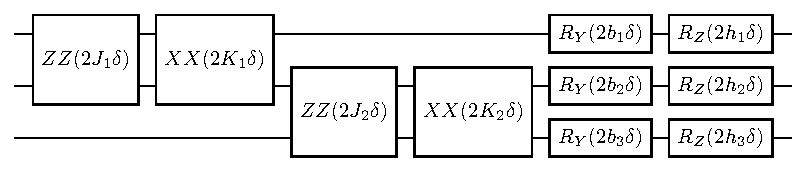
\includegraphics[width=0.52\linewidth]{diagrams/trotter_step.pdf}
\end{tabular}
\caption{The four trial-function architectures, illustrated with three qubits. Shaded blocks repeat $L$ times. Input-dependent gates carry $t$; the remaining angles are trained. Every model reads out $Z_0$.}
\label{fig:circuits}
\end{figure}

\section{Benchmarks}\label{sec:methods}

To benchmark our circuits, we use the following differential equations
\begin{table}[htbp]
\centering\small
\begin{tabularx}{\linewidth}{@{}lXl@{}}
\toprule
Benchmark & Equation in the units used & Window \\
\midrule
Rabi & $P''+P-1/2=0$ & $[0,2\pi]$\\
Damped Rabi & $P''+2\gamma P'+(1+\gamma^2)P-1/2=0$, $\gamma=0.2$ & $[0,5]$\\
Photon decay & $n'+n=0$ & $[0,4]$\\
Two-photon absorption & $I'+I/2+I^2=0$ & $[0,4]$\\
Hermite--Gauss & $\psi''+(3-x^2)\psi=0$ & $[-3,3]$\\
Duffing (``Kerr'') & $x''+x+x^3=0$ & $[0,5]$\\
NLS soliton profile & $u''-u+2u^3=0$ & $[-3,3]$\\
\bottomrule
\end{tabularx}
\caption{ODE test problems from quantum optics~\cite{wallsmilburn2008,boyd2008,kogelnik1966,agrawal,hasegawa1973}, in dimensionless units, with their solution windows.}
\label{tab:problems}
\end{table}
\begin{table}[htbp]
\centering\footnotesize
\begin{tabularx}{\linewidth}{@{}lX@{}}
\toprule
\multicolumn{2}{@{}l}{\textbf{Hardware}}\\
machine & Apple M4, 10 CPU cores (4 performance + 6 efficiency), 16 GB RAM \\
operating system & macOS 26.5.2 \\
\midrule
\multicolumn{2}{@{}l}{\textbf{Software}}\\
language & Python 3.12.12 \\
quantum simulation & PennyLane 0.45.1~\cite{bergholm2018} (\texttt{default.qubit}, \texttt{default.mixed}) \\
autodiff / compilation & JAX and jaxlib 0.10.2 (float64) \\
numerics & NumPy 2.5.4, SciPy 1.18.1, pandas 3.1.0 \\
environment & Nix 2.31.3 flake + uv 0.9.29 \\
\bottomrule
\end{tabularx}
\caption{Compute environment. No accelerator or quantum device was used.}
\label{tab:compute}
\end{table}

\section{Results}\label{sec:results}
Figures~\ref{fig:optics}--\ref{fig:pointwise} and Table~\ref{tab:accuracy} summarize the seven benchmarks.
\begin{figure}[htbp]
\centering
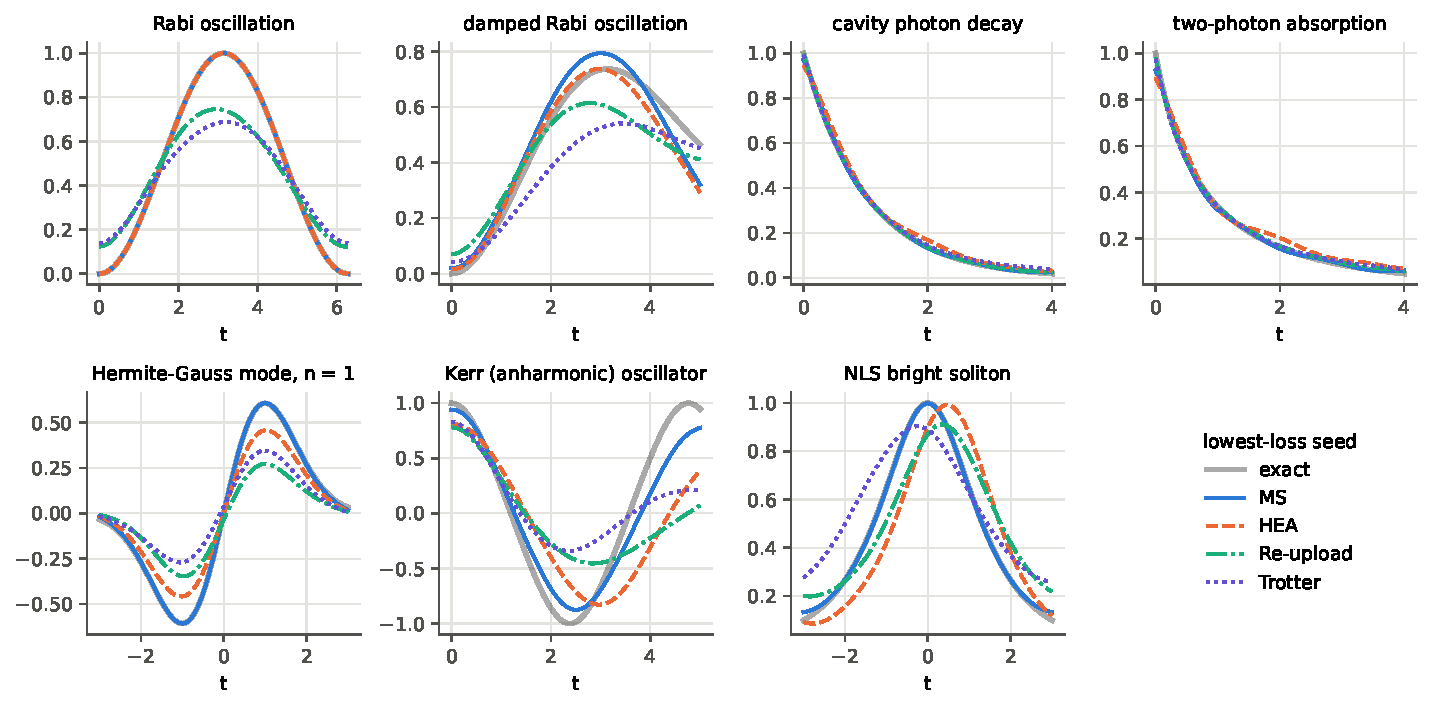
\includegraphics[width=\linewidth]{figures/fig_optics_odes_qubit.pdf}
\caption{Exact reference curves and trained predictions for all seven benchmarks ($n=4$, $L=3$). Each model uses the seed with the lowest final recorded training loss. HEA has fixed depth.}
\label{fig:optics}
\end{figure}
\begin{table}[htbp]
\centering\footnotesize\setlength{\tabcolsep}{4pt}
\begin{tabular}{lrrrr}
\toprule
system & MS & HEA & Re-upload & Trotter \\
\midrule
Rabi oscillation & {\boldmath $1.1\times10^{-8}$} & $1.1\times10^{-4}$ & $2.7\times10^{-1}$ & $3.5\times10^{-1}$ \\
damped Rabi oscillation & {\boldmath $1.1\times10^{-1}$} & $1.2\times10^{-1}$ & $2.6\times10^{-1}$ & $3.3\times10^{-1}$ \\
cavity photon decay & {\boldmath $1.6\times10^{-2}$} & $5.9\times10^{-2}$ & $5.6\times10^{-2}$ & $3.3\times10^{-2}$ \\
two-photon absorption & $3.5\times10^{-2}$ & $8.4\times10^{-2}$ & {\boldmath $2.4\times10^{-2}$} & $7.6\times10^{-2}$ \\
Hermite-Gauss mode, n = 1 & {\boldmath $1.3\times10^{-2}$} & $2.4\times10^{-1}$ & $7.1\times10^{-1}$ & $6.1\times10^{-1}$ \\
Kerr (anharmonic) oscillator & {\boldmath $2.6\times10^{-1}$} & $6.9\times10^{-1}$ & $8.5\times10^{-1}$ & $6.9\times10^{-1}$ \\
NLS bright soliton & {\boldmath $1.6\times10^{-2}$} & $2.6\times10^{-1}$ & $2.9\times10^{-1}$ & $2.7\times10^{-1}$ \\
\midrule
trainable parameters & 45 & 16 & 48 & 42 \\
\bottomrule
\end{tabular}

\caption{Median relative $L^2$ error over three seeds, smallest value per row in bold. Parameter counts are allocated counts and are not matched between models.}
\label{tab:accuracy}
\end{table}

\begin{figure}[htbp]
\centering
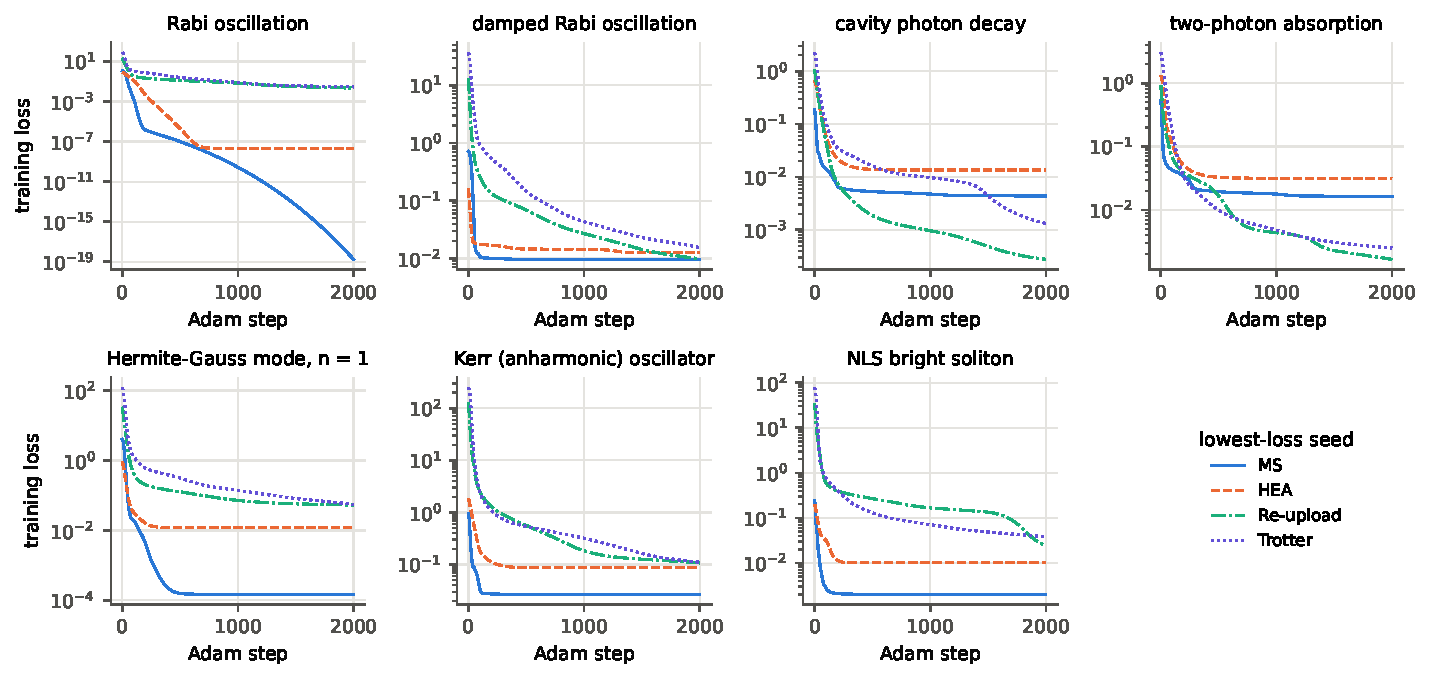
\includegraphics[width=\linewidth]{figures/fig_loss_curves_qubit.pdf}
\caption{Training-objective histories for the selected lowest-final-recorded-loss seed of each architecture on each benchmark.}
\label{fig:loss}
\end{figure}
\begin{figure}[htbp]
\centering
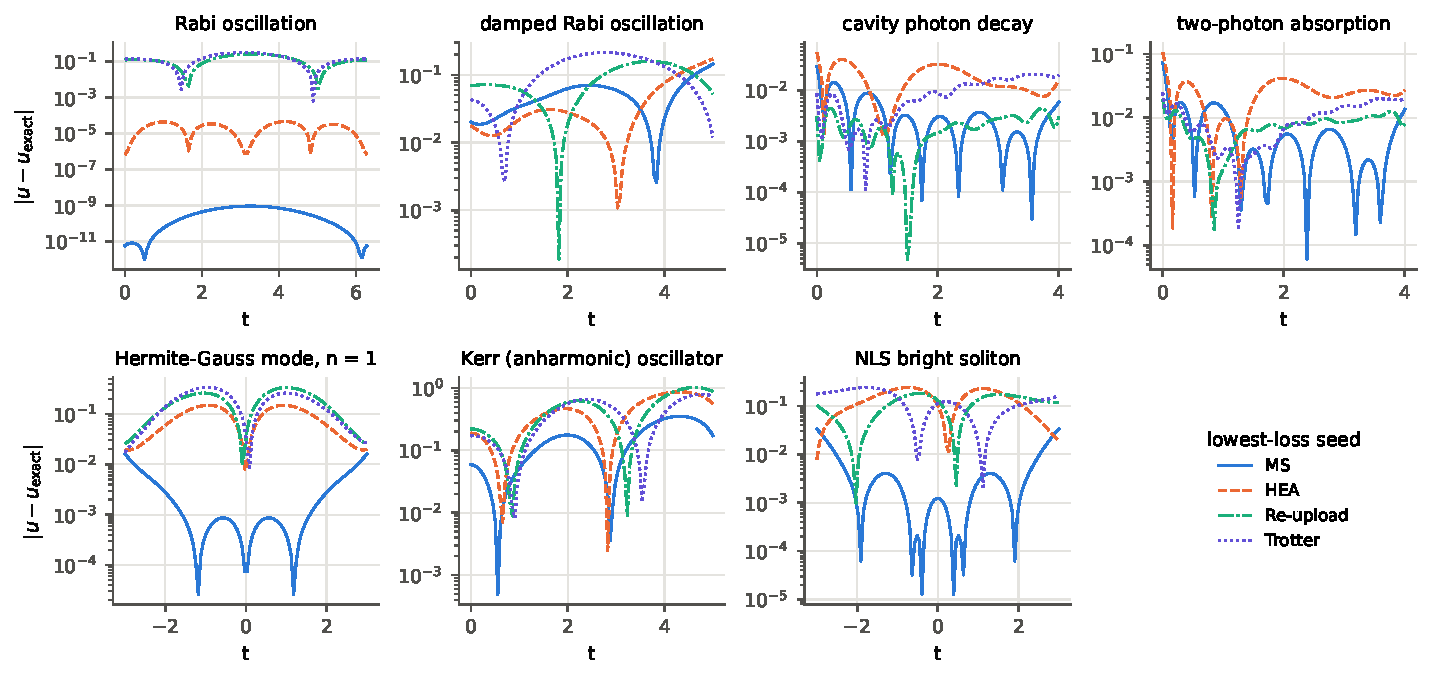
\includegraphics[width=\linewidth]{figures/fig_pointwise_error_qubit.pdf}
\caption{Absolute prediction errors $|u_\theta-u_{\rm exact}|$ for the selected curves in Fig.~\ref{fig:optics}, showing where disagreement occurs within each training window. Values below $10^{-12}$ are displayed at $10^{-12}$ on the logarithmic axis.}
\label{fig:pointwise}
\end{figure}
\FloatBarrier

\section{ODE benchmarks from the literature}\label{sec:litode}

\begin{equation}
    u' + \lambda u(\kappa + \tan\lambda x) = 0, \quad x \in [0, 0.9] \quad \text{\cite{kyriienko2021}}
\end{equation}

\begin{equation}
    u'' + u' + u = 0, \quad t \in [0, 10] \quad \text{\cite{hunout2025}}
\end{equation}

\begin{equation}
    u'' + \sin 4x = 0, \quad x \in [0, \pi/2] \quad \text{\cite{panichi2026}}
\end{equation} 
\begin{figure}[htbp]
\centering
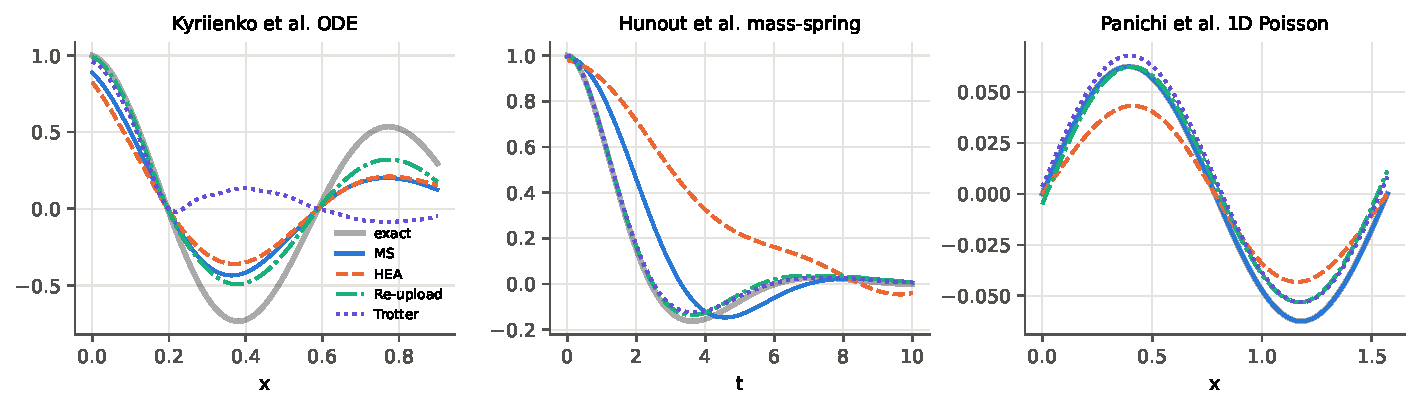
\includegraphics[width=\linewidth]{figures/fig_literature_odes_qubit.pdf}
\caption{Literature ODEs: exact solution and best-loss seed of each circuit.}
\label{fig:litodes}
\end{figure}
\begin{figure}[htbp]
\centering
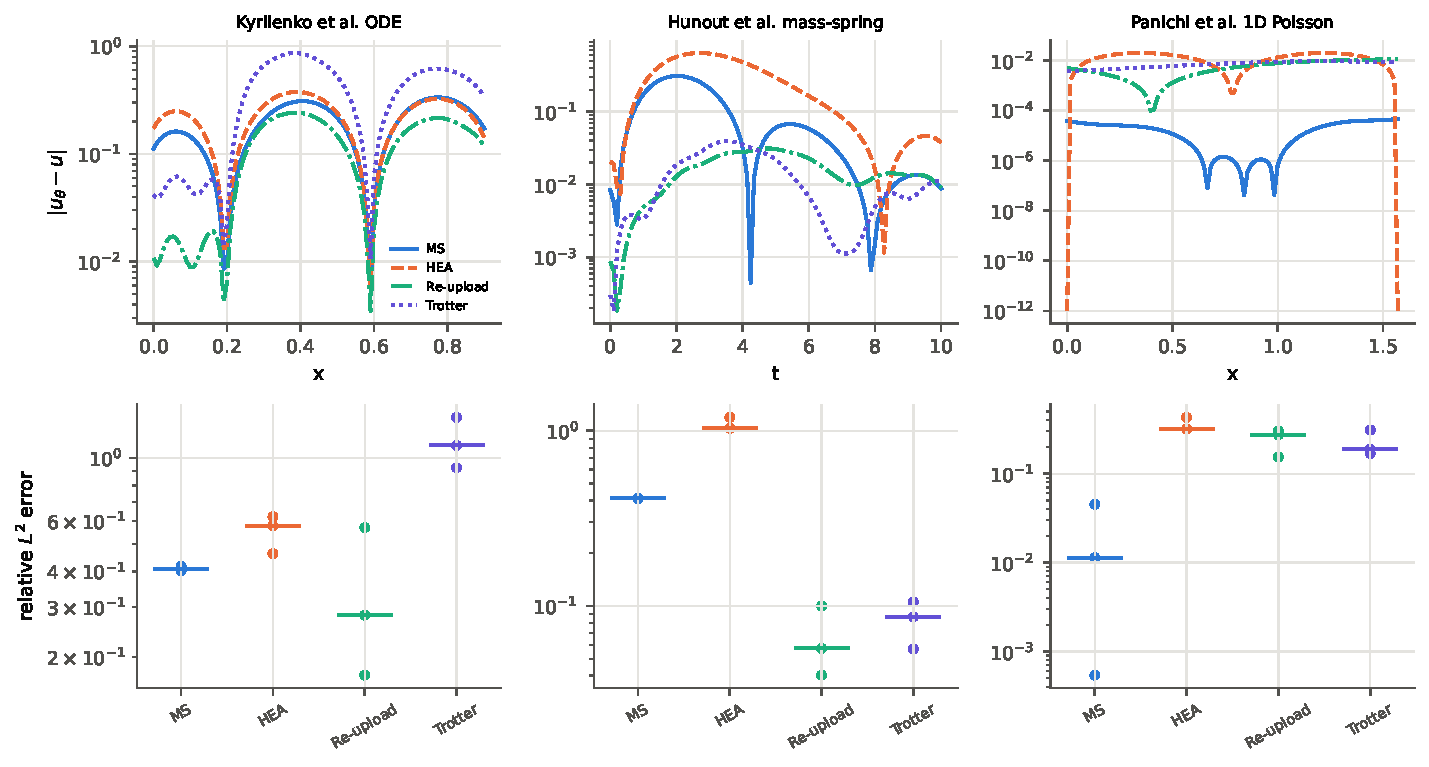
\includegraphics[width=\linewidth]{figures/fig_literature_ode_errors_qubit.pdf}
\caption{Literature ODEs. Top: pointwise error of the best-loss seed. Bottom: error of every seed (dots) and median (bars).}
\label{fig:litodeerr}
\end{figure}
\FloatBarrier

\section{PDE benchmark: the heat equation}\label{sec:pde}
Heat equation of Panichi \emph{et al.}~\cite{panichi2026}:
\begin{equation}
 T_t=0.3\,T_{xx},\qquad x\in[-\tfrac\pi2,\tfrac\pi2],\ t\in[0,0.5],\qquad
 T(x,0)=\tfrac12e^{-(x+\pi/8)^2/0.4},\quad T(\pm\tfrac\pi2,t)=0.
\end{equation}

\begin{figure}[htbp]
\centering
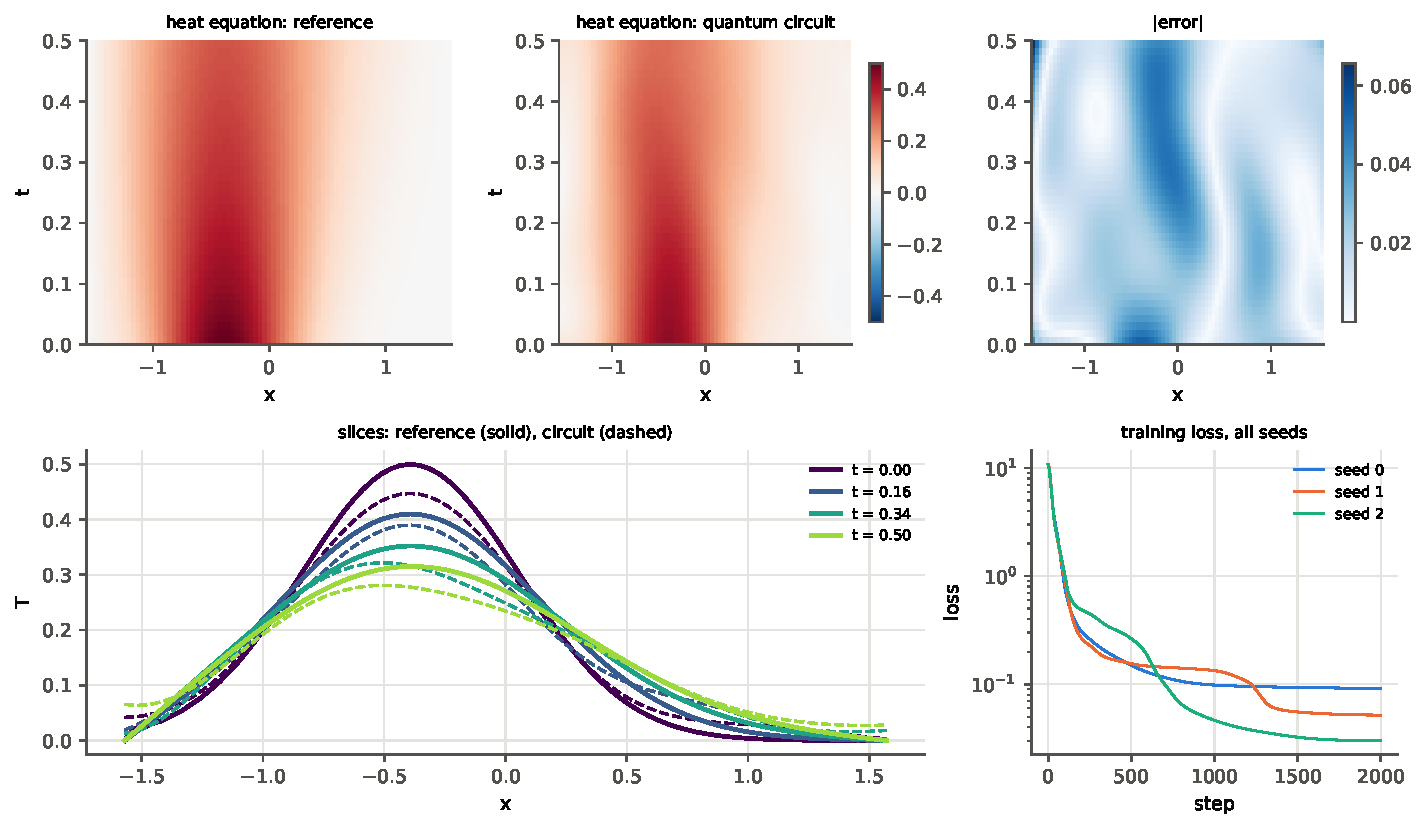
\includegraphics[width=\linewidth]{figures/fig_draft_heat.pdf}
\caption{Heat equation. Top: reference, circuit prediction and error. Bottom: slices at four times and training loss.}
\label{fig:heat}
\end{figure}


\FloatBarrier
\bibliographystyle{unsrtnat}
\bibliography{refs,draft_refs}
\end{document}

